\documentclass[border=10pt]{standalone}
\usepackage[T1]{fontenc}
\usepackage{tikz}
\usepackage{fontawesome5}
\usepackage{amsmath,amssymb}

\usetikzlibrary{calc, positioning, arrows.meta, shapes.geometric, fit, backgrounds}

% ── Modern A* Conference Palette ──
\definecolor{colImgBg}{RGB}{245,247,250}
\definecolor{colImgBorder}{RGB}{185,195,208}

\definecolor{colGSBorder}{RGB}{235,140,85}
\definecolor{colGSEllipse}{RGB}{245,155,100}

\definecolor{colSAMBg}{RGB}{254,249,231}
\definecolor{colSAMBorder}{RGB}{230,190,65}

\definecolor{colSAGABg}{RGB}{244,238,252}
\definecolor{colSAGABorder}{RGB}{186,155,229}

\definecolor{colCLIPBg}{RGB}{236,248,239}
\definecolor{colCLIPBorder}{RGB}{125,195,145}

\definecolor{colCubeEdge}{RGB}{185,195,205}
\definecolor{colCubeFill}{RGB}{250,250,252}

\definecolor{colFire}{RGB}{225,75,35}
\definecolor{colSnow}{RGB}{65,135,200}
\definecolor{colText}{RGB}{35,45,60}
\definecolor{colSubText}{RGB}{100,115,130}
\definecolor{colArr}{RGB}{85,100,120}

% Red spectrum for Gaussians
\definecolor{colGaussLight}{RGB}{242,165,160}  % Light red for context Gaussians
\definecolor{colGaussTarget}{RGB}{215,35,30}   % Deep vibrant red for target cluster

\begin{document}
\sffamily
\begin{tikzpicture}[
    >=Latex,
    font=\sffamily,
    block/.style={
        rounded corners=4pt,
        line width=0.9pt,
        align=center,
        inner sep=4pt,
        text=colText
    },
    arr/.style={->, >=Latex, line width=1.1pt, color=colArr},
    arrDashed/.style={->, >=Latex, line width=1.0pt, dashed, color=colArr},
    lbl/.style={font=\sffamily\scriptsize\itshape, text=colSubText, fill=white, inner sep=1.5pt, rounded corners=2pt}
]

% ════════════════════════════════════════════
% 1. INPUT: Multi-view Images Stack
% ════════════════════════════════════════════
\begin{scope}[shift={(0, 0)}]
    % Frame 3 (Back)
    \fill[colImgBg, draw=colImgBorder, rounded corners=3pt, line width=0.6pt]
        (0.32, 0.32) rectangle ++(1.4, 1.1);
    \draw[colImgBorder!80, line width=0.4pt] (0.42, 1.15) -- (1.45, 1.15);
    \draw[colImgBorder!80, line width=0.4pt] (0.42, 0.95) -- (1.2, 0.95);

    % Frame 2 (Middle)
    \fill[colImgBg, draw=colImgBorder, rounded corners=3pt, line width=0.6pt]
        (0.16, 0.16) rectangle ++(1.4, 1.1);
    \draw[colImgBorder!80, line width=0.4pt] (0.26, 0.99) -- (1.3, 0.99);
    \draw[colImgBorder!80, line width=0.4pt] (0.26, 0.79) -- (1.05, 0.79);

    % Frame 1 (Front)
    \fill[white, draw=colImgBorder!80!black, rounded corners=3pt, line width=0.8pt]
        (0, 0) rectangle ++(1.4, 1.1);
    % Stylized photo content
    \fill[colSubText!25, rounded corners=1.5pt] (0.12, 0.12) rectangle (0.6, 0.6);
    \fill[colGaussTarget!40, rounded corners=1.5pt] (0.75, 0.12) rectangle (1.28, 0.8);
    \draw[colText!30, line width=0.5pt] (0.12, 0.9) -- (1.28, 0.9);

    \node[below, font=\sffamily\bfseries\footnotesize, text=colText] at (0.7, -0.15) {Multi-view};
    \node[below, font=\sffamily\scriptsize, text=colSubText] at (0.7, -0.45) {Images};
\end{scope}

\coordinate (imgOut) at (1.8, 0.55);

% ════════════════════════════════════════════
% 2. 3DGS: Compact Dense Ellipsoid Cluster (no box)
% ════════════════════════════════════════════
\begin{scope}[shift={(4.5, 1.5)}]
    % Clustered anisotropic ellipsoids simulating 3DGS splats
    \fill[colGSEllipse, opacity=0.55] (-0.55, -0.25) ellipse [x radius=0.22, y radius=0.12, rotate=20];
    \fill[colGSEllipse, opacity=0.65] (-0.15, -0.35) ellipse [x radius=0.18, y radius=0.24, rotate=-15];
    \fill[colGSEllipse, opacity=0.75] (0.35, -0.20) ellipse [x radius=0.25, y radius=0.14, rotate=35];
    \fill[colGSEllipse, opacity=0.85] (-0.45, 0.15) ellipse [x radius=0.20, y radius=0.15, rotate=-30];
    \fill[colGSEllipse, opacity=0.90] (0.05, 0.05) ellipse [x radius=0.26, y radius=0.16, rotate=15];
    \fill[colGSEllipse, opacity=0.70] (0.50, 0.10) ellipse [x radius=0.16, y radius=0.22, rotate=-25];
    \fill[colGSEllipse, opacity=0.60] (-0.25, 0.40) ellipse [x radius=0.22, y radius=0.13, rotate=40];
    \fill[colGSEllipse, opacity=0.75] (0.25, 0.38) ellipse [x radius=0.19, y radius=0.14, rotate=-10];

    % Bounding anchor for straight arrows
    \coordinate (gsWest) at (-0.85, 0.05);
    \coordinate (gsEast) at (0.80, 0.05);

    % Title & subtitle
    \node[above, font=\sffamily\bfseries\footnotesize, text=colText] at (0, 0.65)
        {3DGS \textcolor{colFire}{\footnotesize\faFire}};
    \node[below, font=\sffamily\scriptsize, text=colSubText] at (0, -0.55)
        {RGB Gaussians};
\end{scope}

% ════════════════════════════════════════════
% 3. SAM 2: Thinner Vertical Rectangle (Tower)
% ════════════════════════════════════════════
\node[block, fill=colSAMBg, draw=colSAMBorder,
      minimum width=1.15cm, minimum height=2.4cm]
    (sam) at (4.5, -1.2) {
        \textbf{SAM 2}\\[-1pt]
        \textcolor{colSnow}{\footnotesize\faSnowflake}\\[6pt]
        {\scriptsize\textcolor{colSubText}{Temporal}}\\[-1pt]
        {\scriptsize\textcolor{colSubText}{Mask}}\\[-1pt]
        {\scriptsize\textcolor{colSubText}{Propagation}}
    };

% ════════════════════════════════════════════
% 4. SAGA: Contrastive 3D Affinity Field
% ════════════════════════════════════════════
\node[block, fill=colSAGABg, draw=colSAGABorder,
      minimum height=2.3cm, minimum width=2.4cm]
    (saga) at (8.5, 0.55) {
        \textbf{SAGA} \textcolor{colFire}{\footnotesize\faFire}\\[3pt]
        {\scriptsize\textcolor{colSubText}{Contrastive 3D}}\\[-1pt]
        {\scriptsize\textcolor{colSubText}{Affinity Field}}
    };

% ════════════════════════════════════════════
% 5. CLIP: Compact Vertical Trapezoid (Encoder)
% ════════════════════════════════════════════
% A true vertical trapezoid: wider at bottom (input), tapering narrower at top (latent)
\begin{scope}[shift={(8.5, -1.95)}]
    \def\twB{1.6}  % bottom width
    \def\twT{1.0}  % top width
    \def\th{1.3}   % height

    \filldraw[fill=colCLIPBg, draw=colCLIPBorder, line width=0.9pt, rounded corners=2pt]
        (-\twB/2, -\th/2) -- (\twB/2, -\th/2) -- (\twT/2, \th/2) -- (-\twT/2, \th/2) -- cycle;

    \node[align=center, font=\sffamily, text=colText] at (0, 0.05) {
        \textbf{CLIP} \textcolor{colSnow}{\footnotesize\faSnowflake}\\[-2pt]
        {\tiny\textcolor{colSubText}{Encoder}}
    };

    \coordinate (clipNorth) at (0, \th/2);
    \coordinate (clipSouth) at (0, -\th/2);
    \coordinate (clipWest)  at (-\twB/2, 0);
    \coordinate (clipEast)  at (\twB/2, 0);
\end{scope}

% ════════════════════════════════════════════
% 6. OUTPUT: 3D Semantic Gaussians
% ════════════════════════════════════════════
\begin{scope}[shift={(11.8, -0.65)}]
    \def\cx{2.3} \def\cy{2.3} \def\dx{0.75} \def\dy{0.65}

    % Back edges (dashed)
    \draw[colCubeEdge, dashed, line width=0.5pt]
        (\dx, \dy) -- (\cx+\dx, \dy)
        (\dx, \dy) -- (\dx, \cy+\dy);

    % Floor plane
    \fill[colCubeFill!80, opacity=0.5] (0, 0) -- (\cx, 0) -- (\cx+\dx, \dy) -- (\dx, \dy) -- cycle;
    \draw[colCubeEdge, line width=0.6pt] (0, 0) -- (\cx, 0) -- (\cx+\dx, \dy);

    % Side walls
    \fill[colCubeFill!50, opacity=0.3] (0, 0) -- (\dx, \dy) -- (\dx, \cy+\dy) -- (0, \cy) -- cycle;
    \draw[colCubeEdge, line width=0.6pt] (0, 0) -- (0, \cy);
    \draw[colCubeEdge, line width=0.6pt] (\cx, 0) -- (\cx, \cy);
    \draw[colCubeEdge, line width=0.6pt] (\cx+\dx, \dy) -- (\cx+\dx, \cy+\dy);

    % Background Context Gaussians (Light Red)
    \fill[colGaussLight, opacity=0.75] (0.6, 0.65) ellipse [x radius=0.22, y radius=0.13, rotate=25];
    \fill[colGaussLight, opacity=0.70] (1.9, 0.45) ellipse [x radius=0.16, y radius=0.22, rotate=-15];
    \fill[colGaussLight, opacity=0.80] (0.8, 1.85) ellipse [x radius=0.24, y radius=0.14, rotate=40];
    \fill[colGaussLight, opacity=0.75] (2.1, 1.95) ellipse [x radius=0.18, y radius=0.25, rotate=-30];
    \fill[colGaussLight, opacity=0.65] (1.3, 2.25) ellipse [x radius=0.20, y radius=0.11, rotate=10];
    \fill[colGaussLight, opacity=0.70] (0.5, 1.35) ellipse [x radius=0.13, y radius=0.18, rotate=-45];
    \fill[colGaussLight, opacity=0.75] (2.4, 1.15) ellipse [x radius=0.15, y radius=0.20, rotate=15];
    \fill[colGaussLight, opacity=0.65] (2.0, 1.45) ellipse [x radius=0.17, y radius=0.14, rotate=10];

    % Queried Target Gaussians (Deep Vibrant Red: "red chair")
    \fill[colGaussTarget, opacity=0.92] (1.35, 0.95) ellipse [x radius=0.26, y radius=0.16, rotate=20];
    \fill[colGaussTarget, opacity=0.95] (1.65, 1.35) ellipse [x radius=0.21, y radius=0.27, rotate=-20];
    \fill[colGaussTarget, opacity=0.88] (1.10, 1.30) ellipse [x radius=0.19, y radius=0.15, rotate=35];
    \fill[colGaussTarget, opacity=0.92] (1.40, 1.65) ellipse [x radius=0.22, y radius=0.17, rotate=-10];

    % Front Bounding Box Edges
    \draw[colCubeEdge!80!black, line width=0.8pt]
        (0, \cy) -- (\cx, \cy) -- (\cx+\dx, \cy+\dy) -- (\dx, \cy+\dy) -- cycle;
    \draw[colCubeEdge!80!black, line width=0.8pt]
        (0, 0) -- (\cx, 0) -- (\cx, \cy) -- (0, \cy) -- cycle;

    % Caption (Reverted exactly as requested)
    \node[below, font=\sffamily\bfseries\footnotesize, text=colText] at (1.5, -0.2)
        {Semantic 3D Gaussians};
    \node[below, font=\sffamily\scriptsize, text=colSubText] at (1.5, -0.5)
        {(Grouped \& Language-Grounded)};
\end{scope}

\coordinate (cubeIn) at (11.8, 0.55);

% ════════════════════════════════════════════
% 7. STRAIGHT ARROWS ONLY (No Curves)
% ════════════════════════════════════════════

% Images -> 3DGS
\draw[arr] (imgOut) -- (gsWest)
    node[lbl, above=2pt, pos=0.5] {poses};

% Images -> SAM 2
\draw[arr] (imgOut) -- (sam.west |- imgOut)
    node[lbl, below=2pt, pos=0.5] {frames};

% 3DGS -> SAGA (Direct straight line)
\draw[arr] (gsEast) -- (saga.west |- gsEast)
    node[lbl, above=2pt, pos=0.5] {RGB Gaussians};

% SAM 2 -> SAGA (Direct straight line)
\draw[arr] (sam.east |- saga.-145) -- (saga.-145)
    node[lbl, below=2pt, pos=0.4] {masks};

% SAM 2 -> CLIP (Straight orthogonal: down then right)
\draw[arr] (sam.south) |- (clipWest)
    node[lbl, near end, above=2pt] {regions};

% CLIP -> SAGA (Direct straight vertical arrow)
\draw[arrDashed] (clipNorth) -- (saga.south)
    node[lbl, right=2pt, midway] {similarity};

% Text Query -> CLIP (Direct straight horizontal arrow)
\node[font=\sffamily\footnotesize, text=colGaussTarget!90!black, left=1.2cm of clipWest]
    (txt) {``\textit{red chair}''};
\draw[arrDashed] (txt.east) -- (clipWest)
    node[lbl, above=2pt, midway] {query};

% SAGA -> Semantic 3D Gaussians (Direct straight horizontal arrow)
\draw[arr] (saga.east) -- (cubeIn)
    node[lbl, above=2pt, midway] {$f_i \!\in\! \mathbb{R}^{32}$};

\end{tikzpicture}
\end{document}
